
\documentclass[10pt]{beamer}
\usetheme{umbc2}
\useinnertheme{umbcboxes}
\setbeamercolor{umbcboxes}{bg=violet!12,fg=black}

\usepackage{longtable}
\usepackage{tabu}
\usepackage{subeqnar}

\newcommand{\ul}{\underline}
\newcommand{\be}{\begin{equation}}
\newcommand{\ee}{\end{equation}}
\newcommand{\bdm}{\begin{displaymath}}
\newcommand{\edm}{\end{displaymath}}
\newcommand{\bea}{\begin{eqnarray}}
\newcommand{\eea}{\end{eqnarray}}
\newcommand{\bsea}{\begin{subeqnarray*}}
\newcommand{\esea}{\end{subeqnarray*}}
\newcommand{\mb}[1]{\mbox{#1}}
\newcommand{\mc}[3]{\multicolumn{#1}{#2}{#3}}
\newcommand{\bm}[1]{\mbox{\bf #1}}
\newcommand{\bmm}[1]{\mbox{\boldmath$#1$\unboldmath}}
\newcommand{\bmell}{\bmm\ell}
\newcommand{\hateps}{\widehat{\bmm\varepsilon}}
\newcommand{\graybox}[1]{\psboxit{box .9 setgray fill}{\fbox{#1}}}
\newcommand{\mdeg}[1]{\mbox{$#1^{\mbox{\scriptsize o}}$}}
\newcommand{\dd}{\mbox{\footnotesize{$\nabla \! \Delta$}}}
\newcommand{\p}{\partial\,}
\renewcommand{\d}{\mbox{d}}
\newcommand{\dspfrac}{\displaystyle\frac}
\newcommand{\nl}{\\[4mm]}

\title{Processing GNSS Data in Real-Time}

\author{Leo\v{s} Mervart}

\institute{TU Prague}

\date{Frankfurt, January 2014}

% \AtBeginSection[]
% {
%   \begin{frame}
%     \frametitle{Table of Contents}
%     \tableofcontents[currentsection]
%   \end{frame}
% }

\begin{document}

%%%%%%%%%%%%%%%%%%%%%%%%%%%%%%%%%%%%%%%%%%%%%%%%%%%%%%%%%%%%%%%%%%%%%%%%%%%%%%%%

\begin{frame}
  \titlepage
\end{frame}

%%%%%%%%%%%%%%%%%%%%%%%%%%%%%%%%%%%%%%%%%%%%%%%%%%%%%%%%%%%%%%%%%%%%%%%%%%%%%%%%

\begin{frame}
\frametitle{Medieval Times of GNSS (personal memories)}

\begin{description}
\item[1991] Prof. Gerhard Beutler became the director of the Astronomical Institute, University of
  Berne. The so-called Bernese GPS Software started to be used for (post-processing) analyzes of
  GNSS data.
\item[1992] LM started his PhD study at AIUB.
\item[1992] Center for Orbit Determination in Europe (consortium of AIUB, Swisstopo, BKG, IGN, and
  IAPG/TUM) established. Roughly at that time LM met Dr. Georg Weber for the first time.
\item[1993] International GPS Service formally recognized by the IAG.
\item[1994] IGS began providing GPS orbits and other products routinely (January, 1).
\item[1995] GPS declared fully operational.
\end{description}

\end{frame}

%%%%%%%%%%%%%%%%%%%%%%%%%%%%%%%%%%%%%%%%%%%%%%%%%%%%%%%%%%%%%%%%%%%%%%%%%%%%%%%%

\begin{frame}
\frametitle{CODE-Related Works in 1990's}

\begin{itemize}
\item The Bernese GPS Software was the primary tool for CODE analyzes (Fortran~77).
\item IGS reference network was sparse.
\item Real-time data transmission limited (Internet was still young, TCP/IP widely accepted 1989).
\item CPU power of then computers was limited (VAX/VMS OS used at AIUB).
\end{itemize}

In 1990's high precision GPS analyzes were almost exclusively performed in post-processing mode.
The typical precise application of GPS at that time was the processing of a network of static
GPS-only receivers for the estimation of station coordinates.

\end{frame}

%%%%%%%%%%%%%%%%%%%%%%%%%%%%%%%%%%%%%%%%%%%%%%%%%%%%%%%%%%%%%%%%%%%%%%%%%%%%%%%%

\begin{frame}
\frametitle{Tempora mutantur (and maybe ``nos mutamur in illis'')}

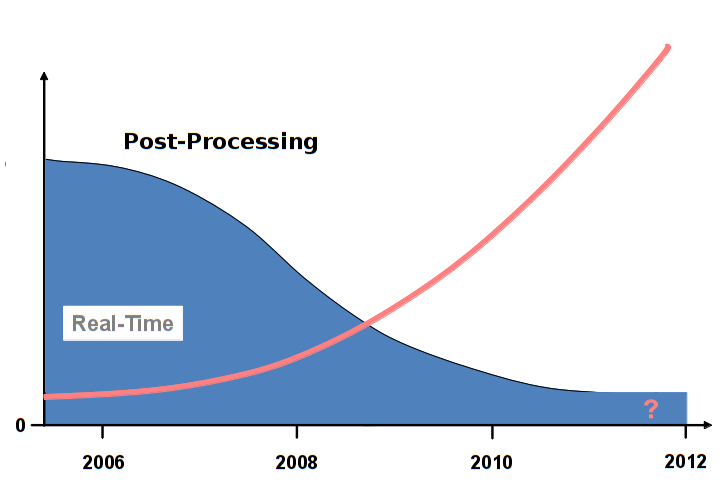
\includegraphics[width=0.7\textwidth,angle=0]{pp_vs_rt.png}

\vspace*{-2cm}
\hspace*{6cm}
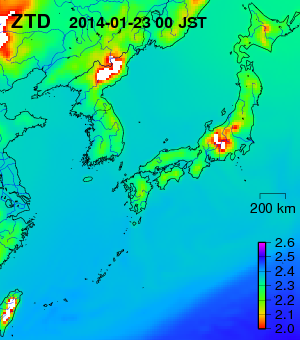
\includegraphics[width=0.4\textwidth,angle=0]{ea_ztd_21h.png}


\end{frame}


%%%%%%%%%%%%%%%%%%%%%%%%%%%%%%%%%%%%%%%%%%%%%%%%%%%%%%%%%%%%%%%%%%%%%%%%%%%%%%%%

\begin{frame}
\frametitle{O tempora! O mores!}

\begin{itemize}
\item people want more and more \ldots
\item everybody wants everything immediately \ldots
\item \hspace*{2cm} and, of course, free of charge \ldots
\end{itemize}
\vspace*{5mm}
In GNSS-world it means:
\begin{itemize}
\item There are many new kinds of GNSS applications - positioning is becoming just one of many
  purposes of GNSS usage.
\item Many results of GNSS processing are required in real-time (or, at least, with very small
  delay).
\item GPS is not the only positioning system. Other GNSS are being established (for practical but
  also for political reasons).
\item People are used that many GNSS services are available free of charge (but the development and
  maintenance has to be funded). 
\end{itemize}

\begin{block}{But \ldots}
\end{block}

\end{frame}

%%%%%%%%%%%%%%%%%%%%%%%%%%%%%%%%%%%%%%%%%%%%%%%%%%%%%%%%%%%%%%%%%%%%%%%%%%%%%%%%

\begin{frame}
\frametitle{Nihil novi sub sole}

Each GNSS-application is based on processing code and/or phase observations
\vspace*{-3mm}
  \begin{eqnarray*}
  P^i & = & \varrho^i + c\;\delta - c\;\delta^i + T^i + I^i + b_P              \\
  L^i & = & \varrho^i + c\;\delta - c\;\delta^i + T^i - I^i + b^i
  \end{eqnarray*}
  where
  \begin{tabbing}
  $P^i$, $L^i$ ~~~~~~~ \= are the code and phase measurements, \\ 
  $\varrho^i$          \> is the travel distance between the satellite 
                          and the receiver,                               \\
  $\delta$, $\delta^i$ \> are the receiver and satellite clock errors,    \\
  $I^i$                \> is the ionospheric delay,                       \\
  $T^i$                \> is the tropospheric delay,                      \\
  $b_P$                \> is the code bias, and                           \\
  $b^i$                \> is the phase bias (including initial
                          phase ambiguity).
  \end{tabbing}
Observation equations reveal what information can be gained from processing GNSS data:
\begin{itemize}
\item geometry (receiver positions, satellite orbits), and
\item state of atmosphere (both dispersive and non-dispersive part)
\end{itemize}
The observation equations also show that, in principle, GNSS is an
\textcolor{blue!90}{interferometric} technique -- precise results are actually always relative.

\end{frame}

%%%%%%%%%%%%%%%%%%%%%%%%%%%%%%%%%%%%%%%%%%%%%%%%%%%%%%%%%%%%%%%%%%%%%%%%%%%%%%%%

\begin{frame}
\frametitle{Challenges of Real-Time GNSS Application}
\begin{itemize}
\item Suitable algorithms for the parameter adjustment have to be used (filter techniques instead
  of classical least-squares).
\item Reliable data links have to been established (between rover station and a reference station,
  between receivers and processing center, or between processing center and DGPS correction
  provider).
\item Software tools for handling real-time data (Fortran is not the best language for that).
\item Fast CPUs.
\end{itemize}

As said above -- GNSS is an interferometric technique. Processing of a single station cannot give
precise results. However, data of reference station(s) can be replaced by the so-called corrections
(DGPS corrections, precise-point positioning etc.) These techniques are particularly suited for
real-time applications because the amount of data being transferred can be considerably reduced.

\end{frame}

%%%%%%%%%%%%%%%%%%%%%%%%%%%%%%%%%%%%%%%%%%%%%%%%%%%%%%%%%%%%%%%%%%%%%%%%%%%%%%%%

\begin{frame}
\frametitle{Algorithms -- Kalman Filter}

\begin{small}

State vectors $\bmm{x}$ at two subsequent epochs are
related to each other by the following linear equation:
\bdm
\bmm{x}(n) = \bmm{\Phi}\; \bmm{x}(n-1) + \bmm{\Gamma}\;\bmm{w}(n)~,
\edm
where $\Phi$ and $\Gamma$ are known matrices and {\em white noise} $\bmm{w}(n)$ is a random
vector with the following statistical properties:
\bsea
E(\bmm{w})                  & = & \bmm{0}                           \\
E(\bmm{w}(n)\;\bmm{w}^T(m)) & = & \bmm{0} ~~ \mbox{for $m \neq n$}  \\
E(\bmm{w}(n)\;\bmm{w^T}(n)) & = & \bm{Q}_s(n) ~.
\esea

Observations $\bmm{l}(n)$ and the state vector $\bmm{x}(n)$ are related to
each other by the linearized {\em observation equations} of form
\bdm \label{eq:KF:obseqn}
 \bmm{l}(n) = \bm{A}\;\bmm{x}(n) + \bmm{v}(n) ~ ,
\edm
where $\bm{A}$ is a known matrix (the so-called {\em first-design matrix}) and
$\bmm{v}(n)$ is a vector of random errors with the following properties:
\bsea\label{eq:KF:resid}
E(\bmm{v})                  & = & \bmm{0} \\
E(\bmm{v}(n)\;\bmm{v}^T(m)) & = & \bmm{0} ~~ \mbox{for $m \neq n$}  \\
E(\bmm{v}(n)\;\bmm{v^T}(n)) & = & \bm{Q}_l(n) ~.
\esea

\end{small}

\end{frame}

%%%%%%%%%%%%%%%%%%%%%%%%%%%%%%%%%%%%%%%%%%%%%%%%%%%%%%%%%%%%%%%%%%%%%%%%%%%%%%%%

\begin{frame}
\frametitle{Classical KF Form}

Minimum Mean Square Error (MMSE) estimate $\widehat{\bmm{x}}(n)$ of vector
$\bmm{x}(n)$ meets the condition
$E\left((\bmm{x} - \widehat{\bmm{x}})(\bmm{x} - \widehat{\bmm{x}})^T\right) =
\mbox{min}$ and is given by
\begin{subeqnarray}\label{eq:KF:prediction}
 \widehat{\bmm{x}}^-(n) & = & \bmm{\Phi} \widehat{\bmm{x}}(n-1)         \\
 \bm{Q}^-(n)            & = & \bmm{\Phi} \bm{Q}(n-1) \bmm{\Phi}^T + 
                          \bmm{\Gamma} \bm{Q}_s(n) \bmm{\Gamma}^T   
\end{subeqnarray}
\begin{subeqnarray}\label{eq:KF:update}
 \widehat{\bmm{x}}(n)   & = & \widehat{\bmm{x}}^-(n) + 
                              \bm{K}\left(\bmm{l} - 
                              \bm{A}\widehat{\bmm{x}}(n-1)\right) \\
 \bm{Q}(n)              & = & \bm{Q}^-(n) - \bm{K}\bm{A}\bm{Q}^-(n) ~,
\end{subeqnarray}
where
\bdm \label{eq:KF:KandH}
 \bm{K} = \bm{Q}^-(n)\bm{A}^T\bm{H}^{-1}, \quad
 \bm{H} = \bm{Q}_l(n) + \bm{A}\bm{Q}^-(n)\bm{A}^T ~.
\edm
Equations (\ref{eq:KF:prediction}) are called {\em prediction}, 
equations (\ref{eq:KF:update}) are called {\em update} step of Kalman filter.

\end{frame}

%%%%%%%%%%%%%%%%%%%%%%%%%%%%%%%%%%%%%%%%%%%%%%%%%%%%%%%%%%%%%%%%%%%%%%%%%%%%%%%%

\begin{frame}
\frametitle{Square-Root Filter} \label{sec:SRF}
\begin{small}
Algorithms based on equations (\ref{eq:KF:prediction}) and
(\ref{eq:KF:update}) may suffer from numerical instabilities that are primarily
caused by the subtraction in (\ref{eq:KF:update}b). This deficiency may be
overcome by the so-called {\em square-root} formulation of the Kalman filter
that is based on the so-called {\em QR-Decomposition}. Assuming the 
Cholesky decompositions
\be \label{eq:SRF:defsym}
  \bm{Q}(n)   = \bm{S}^{T} \bm{S}  , \quad
  \bm{Q}_l(n) = \bm{S}^T_l \bm{S}_l,  \quad
  \bm{Q}^-(n) = \bm{S}^{-T}\bm{S}^- 
\ee
we can create the following block matrix and its QR-Decomposition:
\be \label{eq:SRF:main}
 \left(\begin{array}{ll} 
   \bm{S}_l         & \bm{0} \\
  \bm{S}^-\bm{A}^T  & \bm{S}^-
 \end{array}\right)
=
 N \left(\begin{array}{cc} 
    \bm{X}     & \bm{Y} \\
    \bm{0}     & \bm{Z}
   \end{array}\right) ~ .
\ee
It can be easily verified that 
\bsea\label{eq:SRF:HK}
 \bm{H}    & = & \bm{X}^T\bm{X}   \\
 \bm{K}^T  & = & \bm{X}^{-1}\bm{Y}\\
 \bm{S}    & = & \bm{Z}           \\
 \bm{Q}(n) & = & \bm{Z}^T\bm{Z} ~ .
\esea
State vector $\widehat{\bmm{x}}(n)$ is computed in a usual way using the
equation (\ref{eq:KF:update}a).
\end{small}
\end{frame}

%%%%%%%%%%%%%%%%%%%%%%%%%%%%%%%%%%%%%%%%%%%%%%%%%%%%%%%%%%%%%%%%%%%%%%%%%%%%%%%%

\begin{frame}
\frametitle{Data Transfer -- NTRIP}

In order to be useful data have to be provided in a well-defined \textcolor{blue}{format}.
RTCM (Radio Technical Commission for Maritime Services) messages are widely used for GNSS data in
real-time. 

\vspace*{5mm}

In addition to a format the so-called \textcolor{blue}{protocol} has to be defined. Using a given
protocol the data user communicates with the data provider.

For GNSS data, the so-called \textcolor{blue}{NTRIP} streaming protocol is used.
\begin{itemize}
\item NTRIP stands for Networked Transport of RTCM via Internet Protocol.
\item NTRIP is in principle a layer on top of TCP/IP.
\item NTRIP has been developed at BKG (together with TU Dortmund).
\item NTRIP is capable of handling hundreds of data streams simultaneously delivering the data
to thousands of users.
\item NTRIP is world-wide accepted (great success of BKG).
\end{itemize}

\end{frame}

%%%%%%%%%%%%%%%%%%%%%%%%%%%%%%%%%%%%%%%%%%%%%%%%%%%%%%%%%%%%%%%%%%%%%%%%%%%%%%%%

\begin{frame}
\frametitle{NTRIP}

Efficiency of data transfer using NTRIP is achieved thanks to the GNSS Internet Radio /
IP-Streaming architecture:

\begin{center}
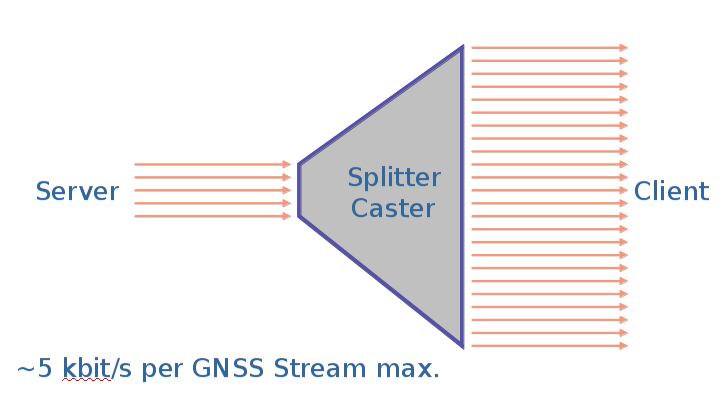
\includegraphics[width=0.7\textwidth,angle=0]{ntrip.png}
\end{center}

\end{frame}

%%%%%%%%%%%%%%%%%%%%%%%%%%%%%%%%%%%%%%%%%%%%%%%%%%%%%%%%%%%%%%%%%%%%%%%%%%%%%%%%

\begin{frame}
\frametitle{NTRIP Users}

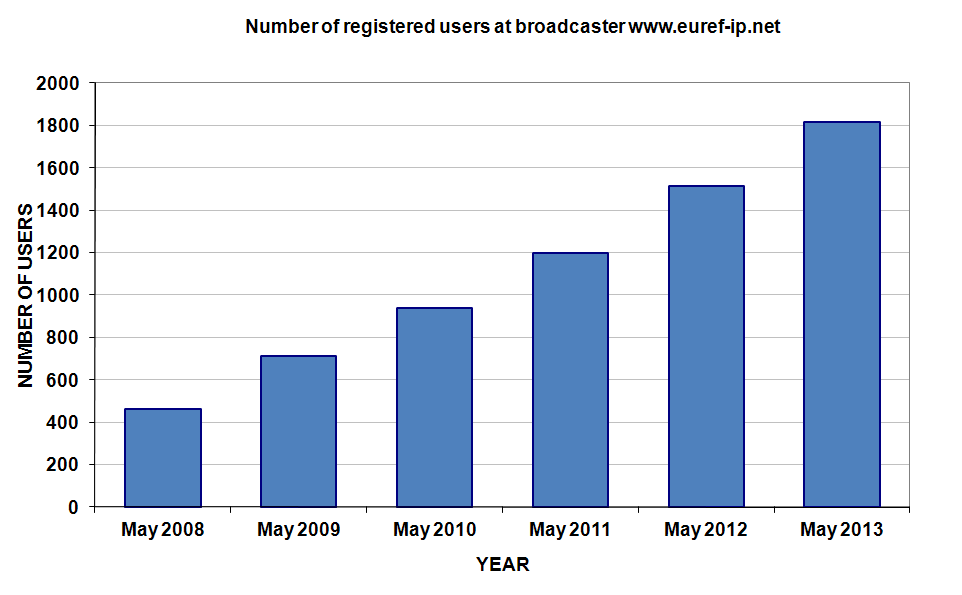
\includegraphics[width=0.5\textwidth,angle=0]{numberRegisteredUsers_1.png}
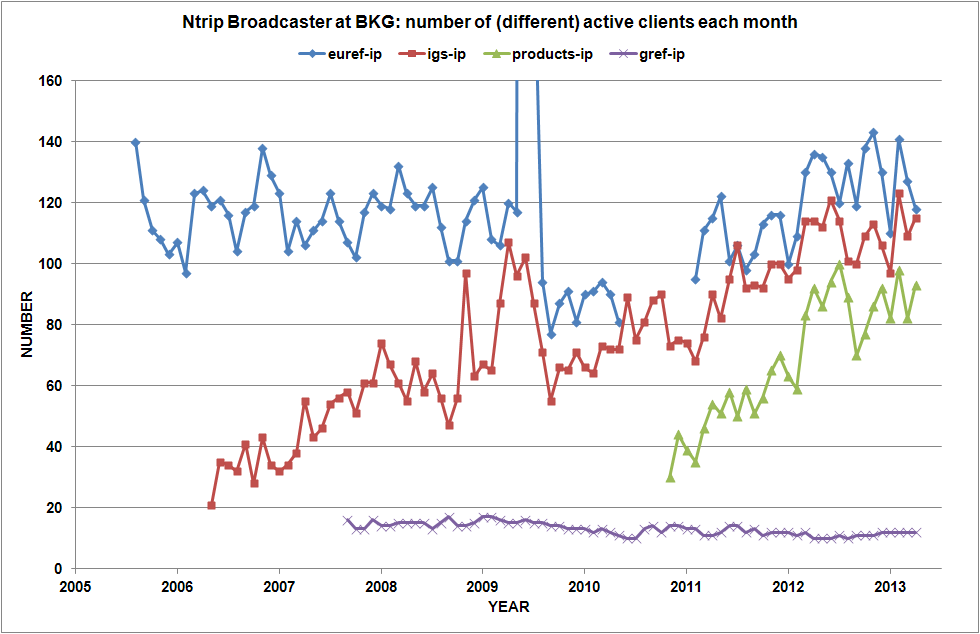
\includegraphics[width=0.5\textwidth,angle=0]{activeClients_month_1.png}
\begin{center}
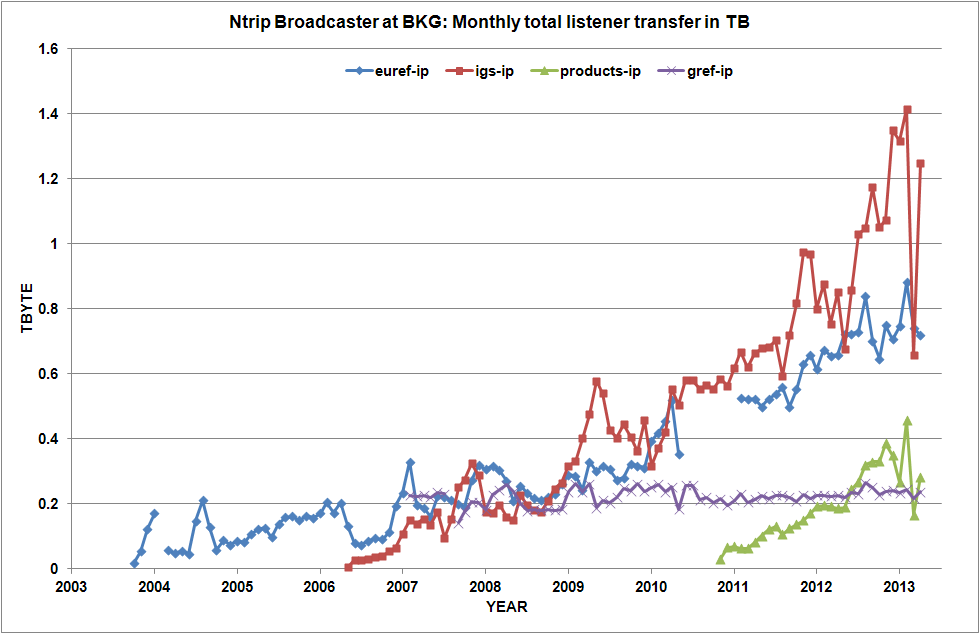
\includegraphics[width=0.5\textwidth,angle=0]{casterTransfer_1.png}
\end{center}

\end{frame}

%%%%%%%%%%%%%%%%%%%%%%%%%%%%%%%%%%%%%%%%%%%%%%%%%%%%%%%%%%%%%%%%%%%%%%%%%%%%%%%%

\begin{frame}
\frametitle{BKG Ntrip Client (BNC)}

An important reason why NTRIP has been widely accepted is that BKG provided high-quality public
license software tools for its usage. One of these tools is the so-called \textcolor{blue}{BKG
Ntrip Client}.

  \begin{itemize}
  \item BNC source consists currently of approximately 50.000 lines of code 
  \item development started 2005 (LM and Georg Weber)
  \item BNC uses a few third-party pieces of software (e.g. RTCM decoders/encoders)
  \item BNC has a good documentation (thanks Georg Weber)
  \end{itemize}

  \begin{block}{BNC is intended to be}
  \begin{itemize}
  \item user-friendly
  \item cross-platform
  \item easily modifiable (by students, GNSS beginners)
  \item useful (at least a little bit ...)
  \end{itemize}
  \end{block}

  \begin{block}{BNC is not only an NTRIP client \ldots}
  \end{block}

\end{frame}

%%%%%%%%%%%%%%%%%%%%%%%%%%%%%%%%%%%%%%%%%%%%%%%%%%%%%%%%%%%%%%%%%%%%%%%%%%%%%%%%

\begin{frame}
\frametitle{BNC Basic Usage}
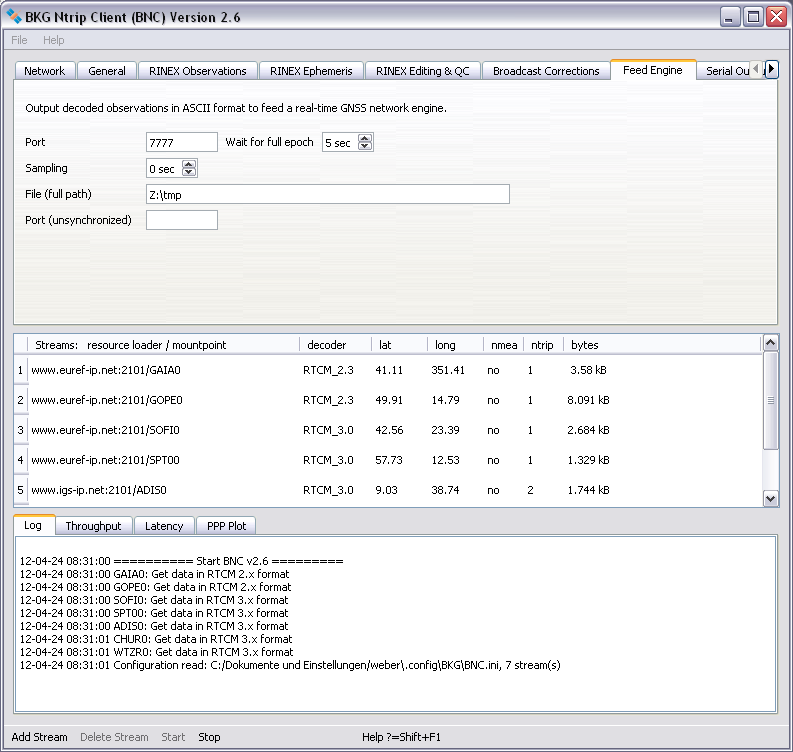
\includegraphics[width=0.6\textwidth,angle=0]{screenshot12.png}

\vspace*{-4cm}
\hspace*{4cm}
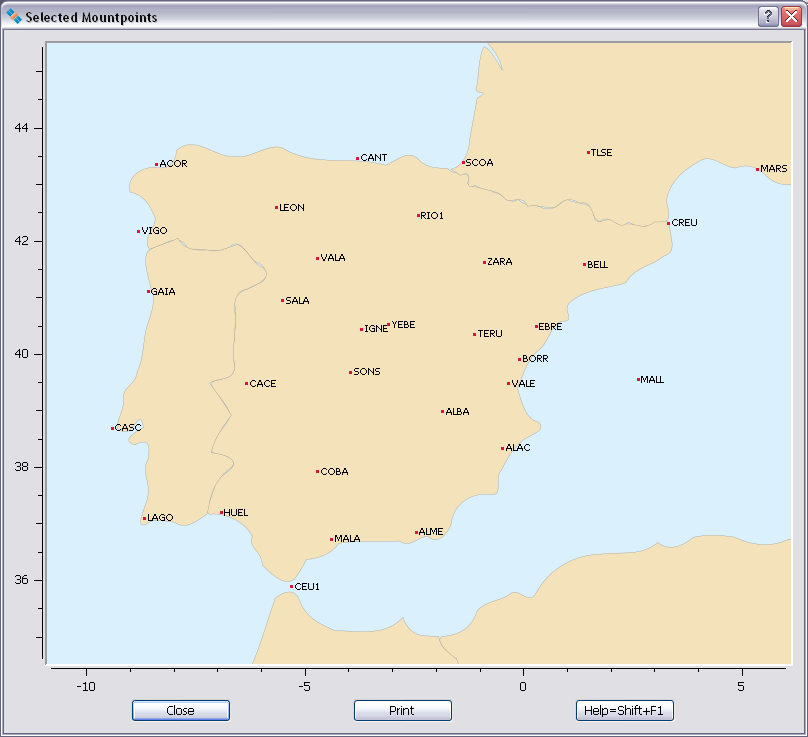
\includegraphics[width=0.5\textwidth,angle=0]{screenshot24.png}
\end {frame}

%%%%%%%%%%%%%%%%%%%%%%%%%%%%%%%%%%%%%%%%%%%%%%%%%%%%%%%%%%%%%%%%%%%%%%%%%%%%%%%%

\begin{frame}
  \frametitle{Data QC in BNC}
  \begin{center}
    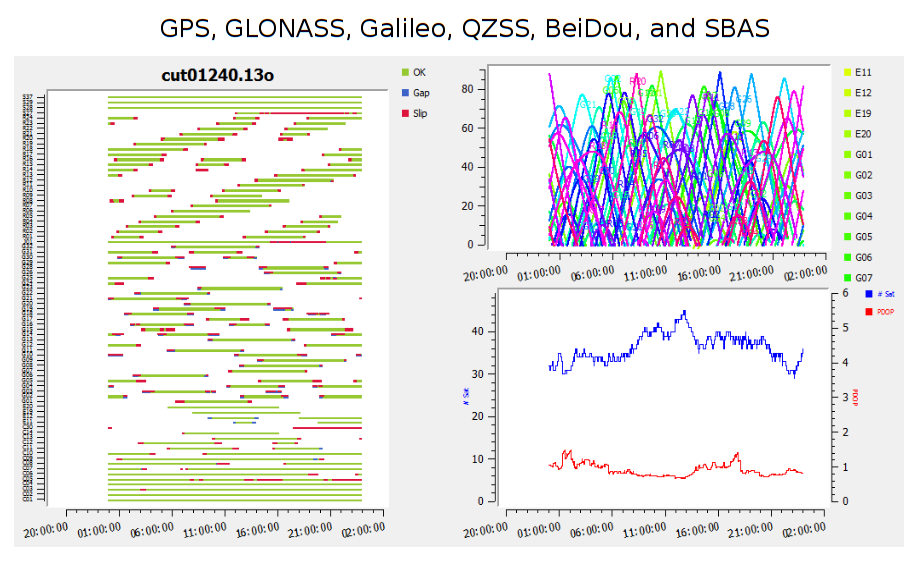
\includegraphics[width=0.9\textwidth,angle=0]{bnc_qc2.png}
  \end{center}
\end {frame}

%%%%%%%%%%%%%%%%%%%%%%%%%%%%%%%%%%%%%%%%%%%%%%%%%%%%%%%%%%%%%%%%%%%%%%%%%%%%%%%%

\begin{frame}
  \frametitle{Data QC in BNC}
  \begin{center}
    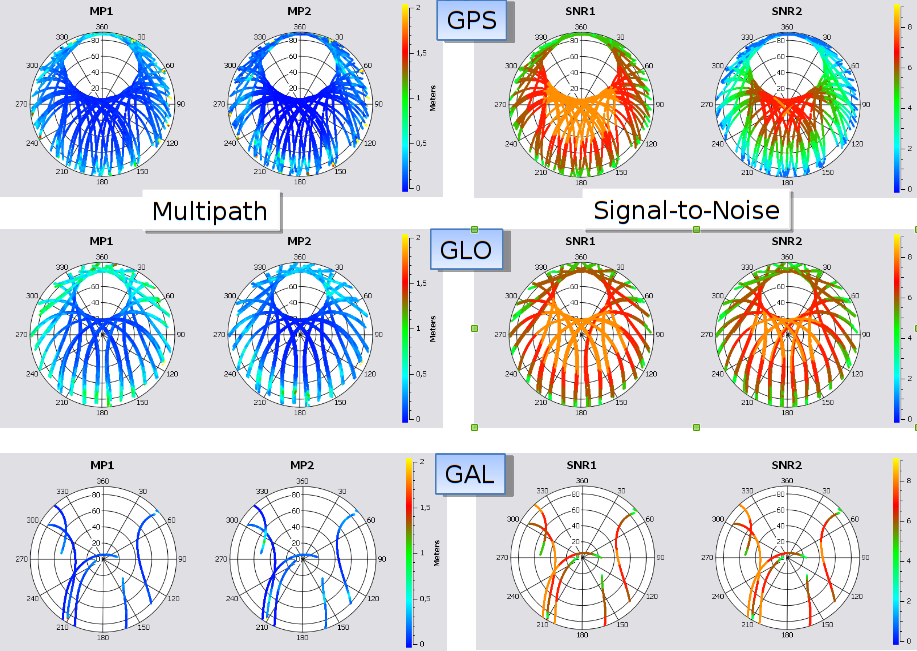
\includegraphics[width=0.9\textwidth,angle=0]{bnc_qc1.png}
  \end{center}
\end {frame}

%%%%%%%%%%%%%%%%%%%%%%%%%%%%%%%%%%%%%%%%%%%%%%%%%%%%%%%%%%%%%%%%%%%%%%%%%%%%%%%%

\begin{frame}
  \frametitle{Precise Point Positioning with PPP}
  \begin{center}
    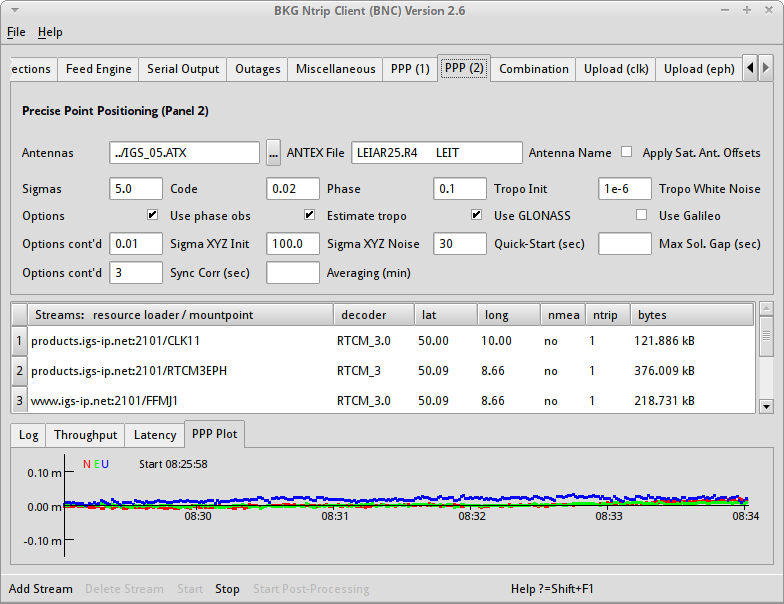
\includegraphics[width=0.9\textwidth,angle=0]{ppp1.png}
  \end{center}
\end {frame}

%%%%%%%%%%%%%%%%%%%%%%%%%%%%%%%%%%%%%%%%%%%%%%%%%%%%%%%%%%%%%%%%%%%%%%%%%%%%%%%%

\begin{frame}
\frametitle{Principles of Precise Point Positioning}
\framesubtitle{Observation Equations}

The PPP is based on the processing of the ionosphere-free linear combination of phase
observations
\be
L^{ij}_3 = \varrho^{ij} - c\delta^{ij} + T^{ij} + \bar{N}^{ij}_3 ~,
\ee 
where the ambiguity term is given by
\be
\bar{N}^{ij}_3 =  N^{ij}_3 - l^{ij}_3 
              = \frac{c\;f_2}{f^2_1-f^2_2}\;(n^{ij}_1-n^{ij}_2) + \lambda_3\;n^{ij}_1 - l^{ij}_3 
\ee
and (optionally) the ionosphere-free linear combination of code observations
\be
P^{ij}_3 = \varrho^{ij} - c\delta^{ij} + T^{ij} + p^{ij}_3 ~,
\ee
where the code bias $p^{ij}_3$ is the linear combination of biases
$p^{ij}_1,p^{ij}_2$
\end{frame}

%%%%%%%%%%%%%%%%%%%%%%%%%%%%%%%%%%%%%%%%%%%%%%%%%%%%%%%%%%%%%%%%%%%%%%%%%%%%%%%%

\begin{frame}
\frametitle{Principles of PPP Service}

The server has to provide the orbit corrections and the satellite clock corrections
$c\delta^{ij}$. That is sufficient for a client processing phase observations only. 

Using the code observations on the client-side is not mandatory. After an initial convergence
period (tens of minutes) there is almost no difference between a phase-only client and the client
that uses also the code observations. However, correct utilization of accurate code observations
improves the positioning results during the convergence period.

Client which processes code observations either
\begin{enumerate}
\item has to know the value $p^{ij}_3$ (the value must be provided by the server -- the most
  correct approach), or
\item has to estimate terms $p^{ij}_3$, or
\item neglect the bias (de-weight the code observations -- not fully correct).
\end{enumerate}
Options (2) and (3) mean that the benefit of using the code observations on the client-side (in
addition to phase observations) is minor only. 

\end{frame}

%%%%%%%%%%%%%%%%%%%%%%%%%%%%%%%%%%%%%%%%%%%%%%%%%%%%%%%%%%%%%%%%%%%%%%%%%%%%%%%%

\begin{frame}
  \frametitle{PPP Options in BNC}
  \begin{itemize}
  \item single station, SPP or PPP
  \item real-time or post-processing
  \item processing of code and phase ionosphere-free combinations, GPS,
    Glonass, and Galileo
  \end{itemize}
  \begin{center}
    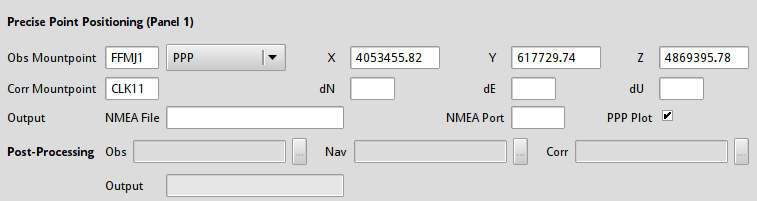
\includegraphics[width=0.9\textwidth,angle=0]{ppp_opt1.png} \\[2mm]
    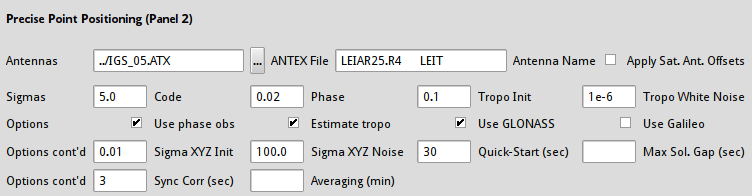
\includegraphics[width=0.9\textwidth,angle=0]{ppp_opt2.png}
  \end{center}
\end {frame}

%%%%%%%%%%%%%%%%%%%%%%%%%%%%%%%%%%%%%%%%%%%%%%%%%%%%%%%%%%%%%%%%%%%%%%%%%%%%%%%%

\begin{frame}
\frametitle{PPP of Moving Receiver by BNC}
  \begin{center}
    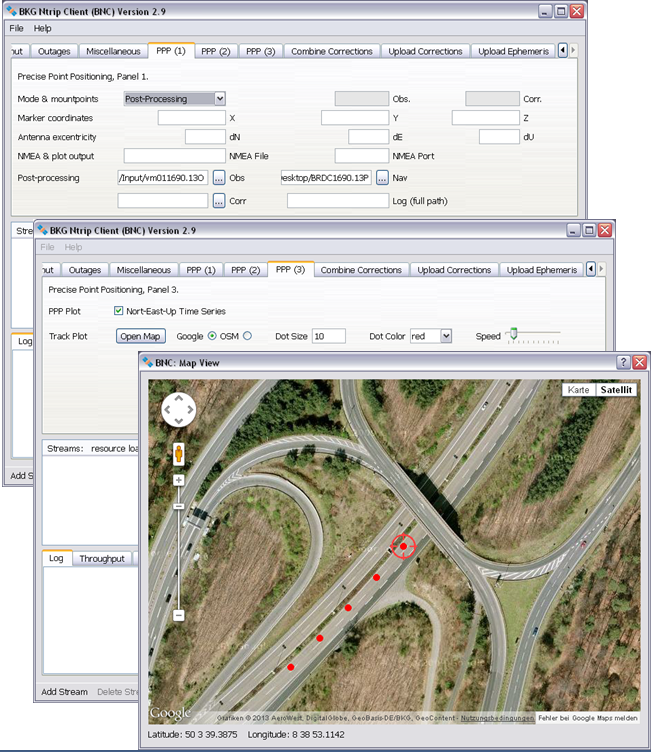
\includegraphics[width=0.6\textwidth,angle=0]{screenshot32.png}
  \end{center}
\end{frame}

%%%%%%%%%%%%%%%%%%%%%%%%%%%%%%%%%%%%%%%%%%%%%%%%%%%%%%%%%%%%%%%%%%%%%%%%%%%%%%%%

\begin{frame}
\frametitle{PPP -- Server-Side}

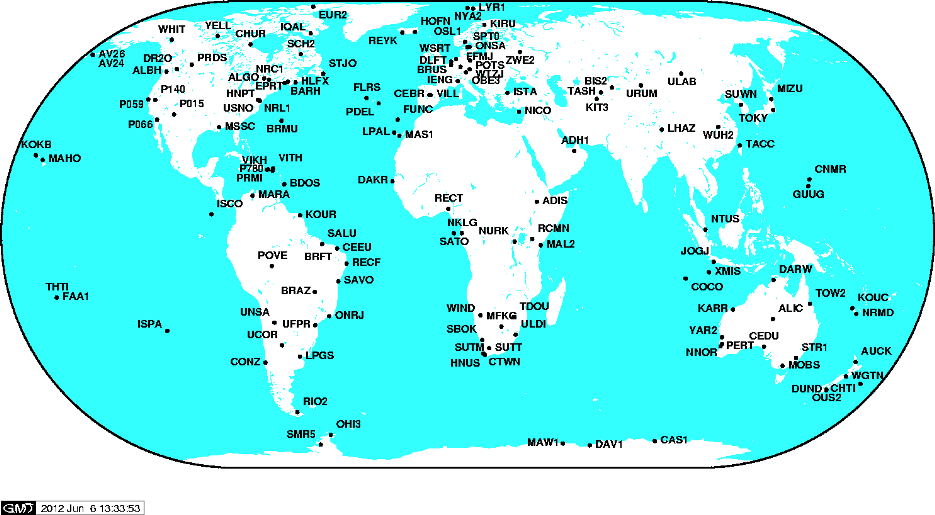
\includegraphics[width=0.8\textwidth,angle=0]{igs_map.png}

\vspace*{-2cm}

\hspace*{2cm}
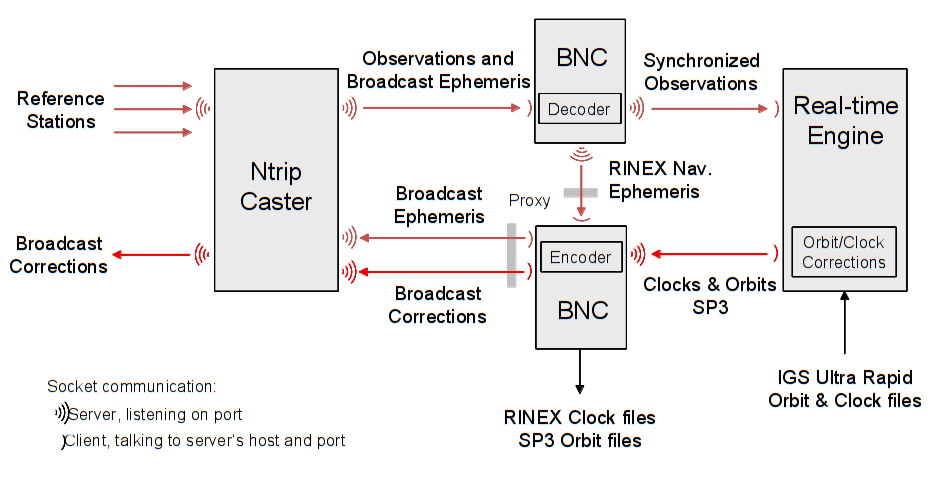
\includegraphics[width=0.8\textwidth,angle=0]{bnc_rtnet_flow.png}

\end{frame}

%%%%%%%%%%%%%%%%%%%%%%%%%%%%%%%%%%%%%%%%%%%%%%%%%%%%%%%%%%%%%%%%%%%%%%%%%%%%%%%%

\begin{frame}
\frametitle{PPP -- Server-Side}
  \begin{center}
    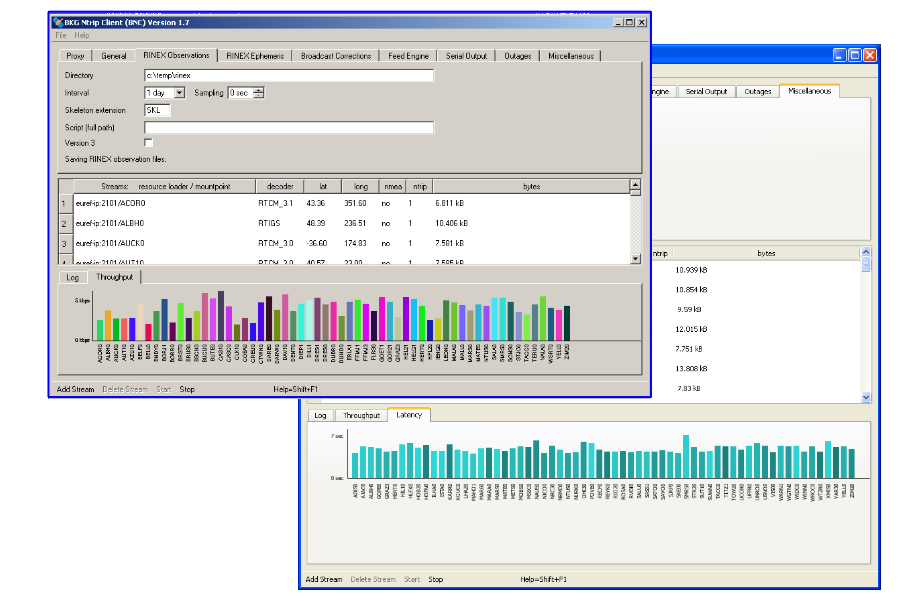
\includegraphics[width=0.9\textwidth,angle=0]{bnc_feed.png}
  \end{center}
\end{frame}

%%%%%%%%%%%%%%%%%%%%%%%%%%%%%%%%%%%%%%%%%%%%%%%%%%%%%%%%%%%%%%%%%%%%%%%%%%%%%%%%

\begin{frame}
\frametitle{PPP -- Server-Side}
  \begin{center}
    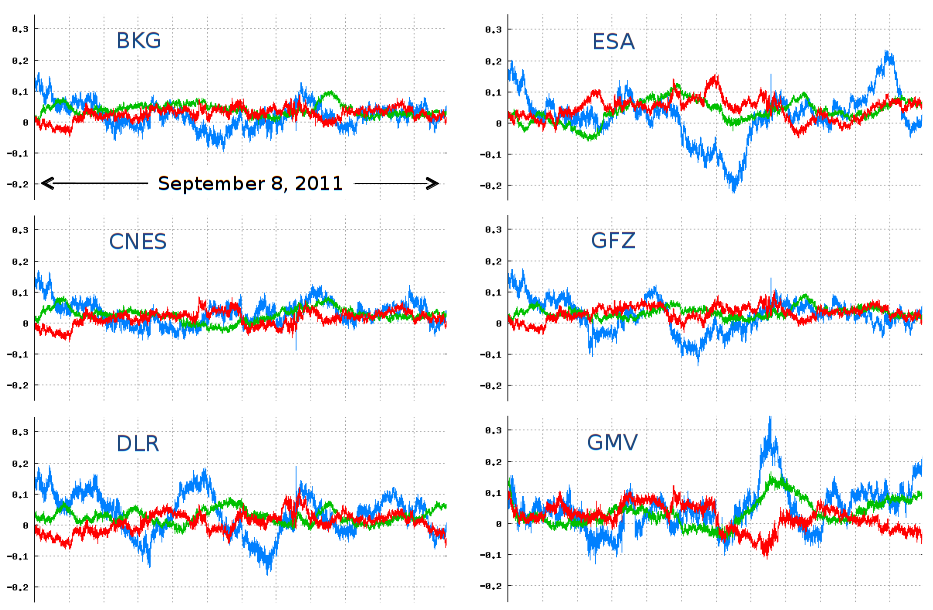
\includegraphics[width=0.9\textwidth,angle=0]{ac_results.png}
  \end{center}
\end{frame}

%%%%%%%%%%%%%%%%%%%%%%%%%%%%%%%%%%%%%%%%%%%%%%%%%%%%%%%%%%%%%%%%%%%%%%%%%%%%%%%%

\begin{frame}
\frametitle{PPP -- Server-Side}
  \begin{center}
    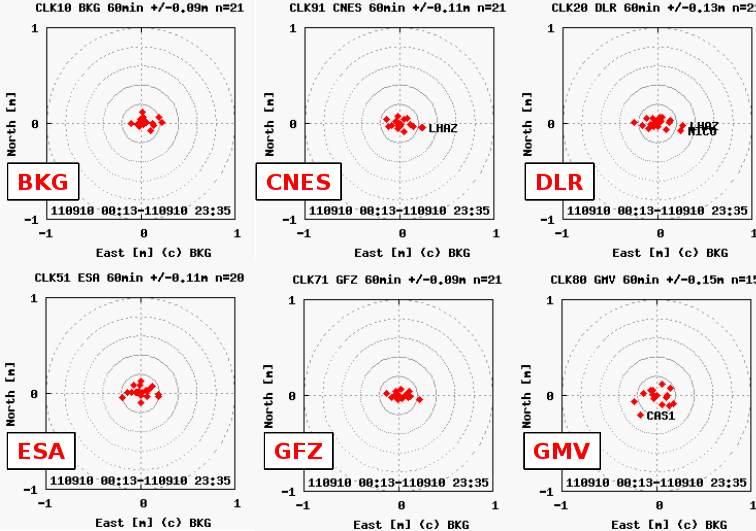
\includegraphics[width=0.9\textwidth,angle=0]{ac_results2.png}
  \end{center}
\end{frame}

%%%%%%%%%%%%%%%%%%%%%%%%%%%%%%%%%%%%%%%%%%%%%%%%%%%%%%%%%%%%%%%%%%%%%%%%%%%%%%%%

\begin{frame}
  \frametitle{Combination using Kalman filtering}
  The combination is performed in two steps
  \begin{itemize}
  \item[1.] The satellite clock corrections that refer to different broadcast
    messages (different IODs) are modified in such a way that they all refer
    to common broadcast clock value (common IOD is that of the selected
    ``master'' analysis center).
  \item[2.] The corrections are used as pseudo-observations for Kalman filter
    using the following model (observation equation):
    \begin{displaymath}
    c_a^s = c^s + o_a + o_a^s
    \end{displaymath}
    where
    \begin{tabbing}
    $c_a^s$ ~~ \= is the clock correction for satellite s estimated by \\
               \> the analysis center a, \\
    $c^s$      \> is the resulting (combined) clock correction for 
                  satellite s, \\
    $o_a$      \> is the AC-specific offset 
                  (common for all satellites), and \\
    $o_a^s$      \> is the satellite and AC-specific offset.
    \end{tabbing}
  \end{itemize}
  The three types of unknown parameters $c^s$, $o_a$, $o_a^s$ differ in their
  stochastic properties: the parameters $c^s$ and $o_a$ are considered to be
  epoch-specific while the satellite and AC-specific offset $o_a^s$ is assumed
  to be a static parameter.
\end{frame}

%%%%%%%%%%%%%%%%%%%%%%%%%%%%%%%%%%%%%%%%%%%%%%%%%%%%%%%%%%%%%%%%%%%%%%%%%%%%%%%%

\begin{frame}
\frametitle{PPP -- Server-Side}
  \begin{center}
    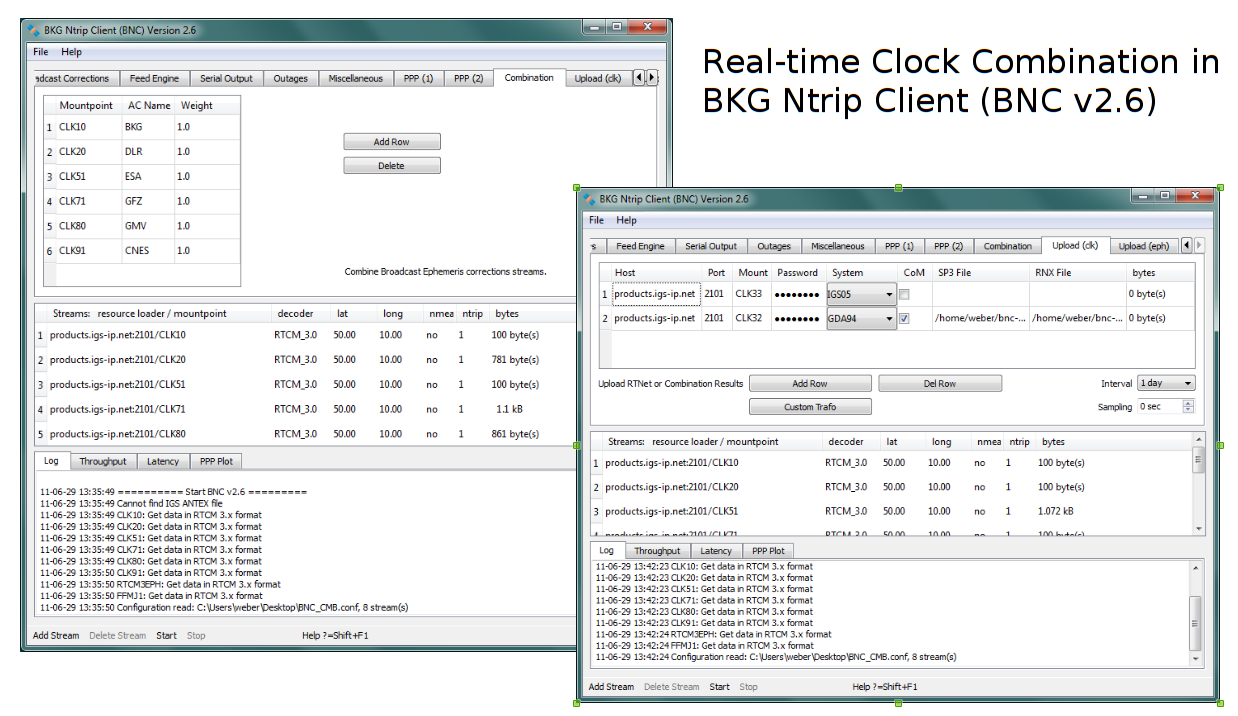
\includegraphics[width=0.9\textwidth,angle=0]{combination_1.png}
  \end{center}
\end{frame}

%%%%%%%%%%%%%%%%%%%%%%%%%%%%%%%%%%%%%%%%%%%%%%%%%%%%%%%%%%%%%%%%%%%%%%%%%%%%%%%%

\begin{frame}
\frametitle{PPP -- Server-Side}
  \begin{center}
    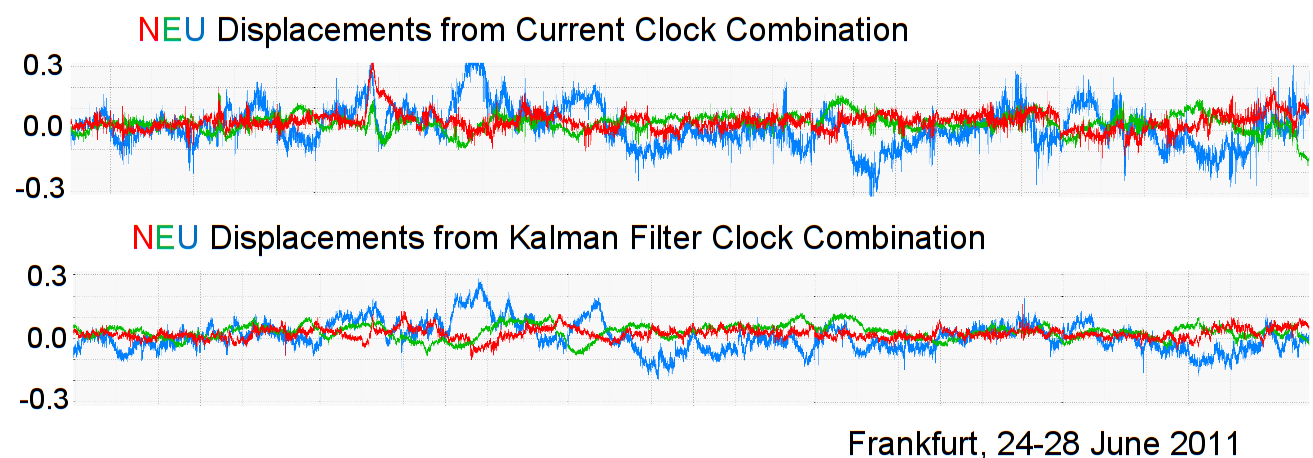
\includegraphics[width=0.9\textwidth,angle=0]{combination_2.png}
  \end{center}
\end{frame}

%%%%%%%%%%%%%%%%%%%%%%%%%%%%%%%%%%%%%%%%%%%%%%%%%%%%%%%%%%%%%%%%%%%%%%%%%%%%%%%%

\begin{frame}
\frametitle{PPP -- Server-Side}
  \begin{center}
    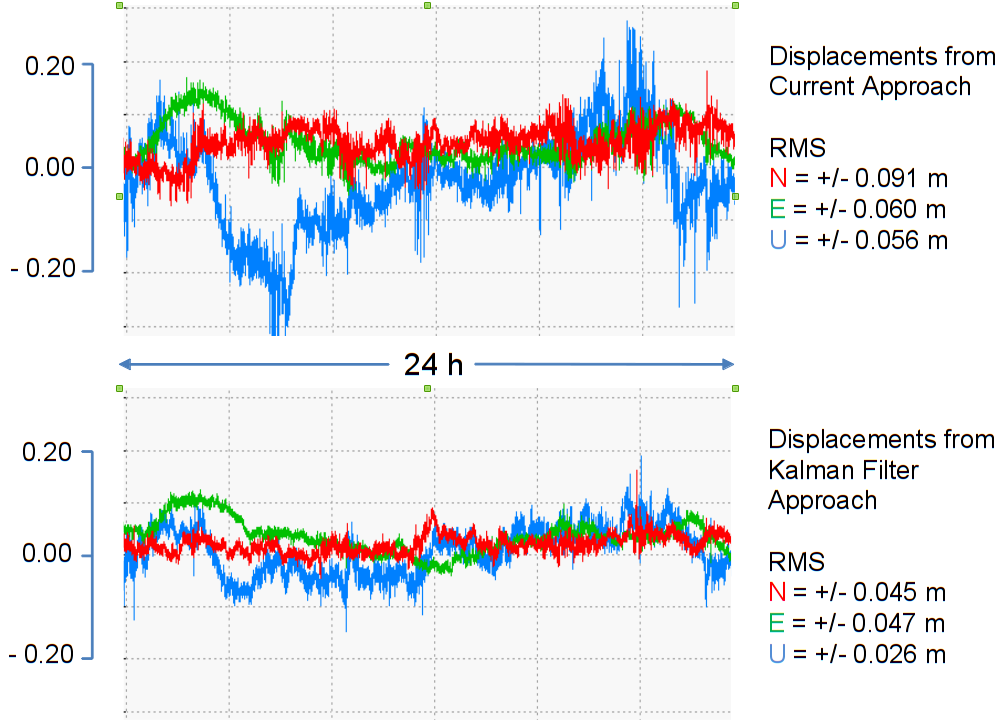
\includegraphics[width=0.9\textwidth,angle=0]{combination_3.png}
  \end{center}
\end{frame}

%%%%%%%%%%%%%%%%%%%%%%%%%%%%%%%%%%%%%%%%%%%%%%%%%%%%%%%%%%%%%%%%%%%%%%%%%%%%%%%%

\begin{frame}
\frametitle{PPP -- Server-Side}
  \begin{center}
    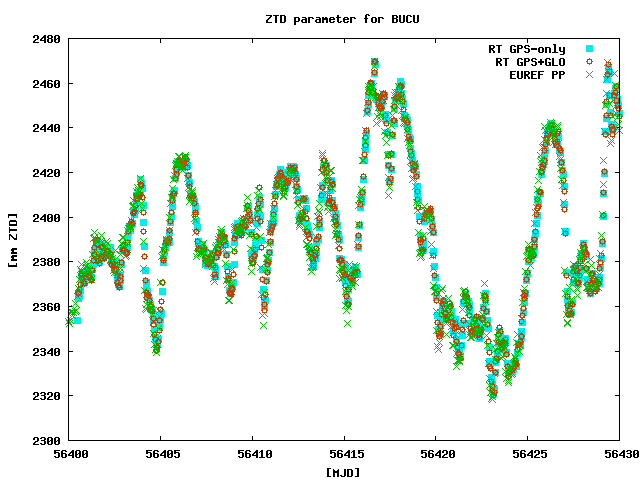
\includegraphics[width=0.9\textwidth,angle=0]{tropo1.png}
  \end{center}
\end{frame}

%%%%%%%%%%%%%%%%%%%%%%%%%%%%%%%%%%%%%%%%%%%%%%%%%%%%%%%%%%%%%%%%%%%%%%%%%%%%%%%%

\begin{frame}
\frametitle{PPP -- Server-Side}
  \begin{center}
    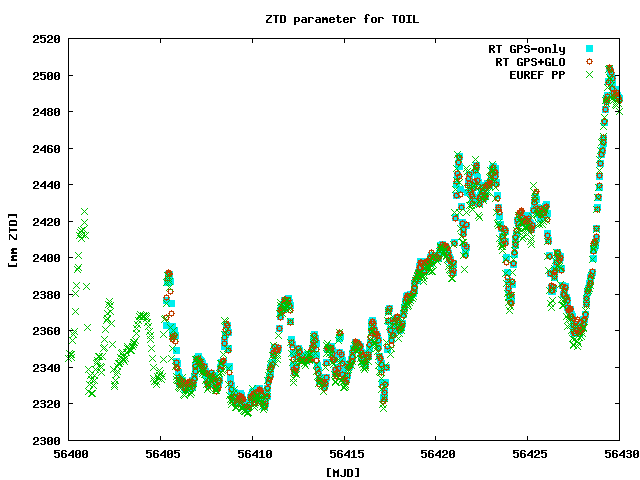
\includegraphics[width=0.9\textwidth,angle=0]{tropo2.png}
  \end{center}
\end{frame}

%%%%%%%%%%%%%%%%%%%%%%%%%%%%%%%%%%%%%%%%%%%%%%%%%%%%%%%%%%%%%%%%%%%%%%%%%%%%%%%%

\begin{frame}
\frametitle{PPP -- Server-Side}
  \begin{center}
    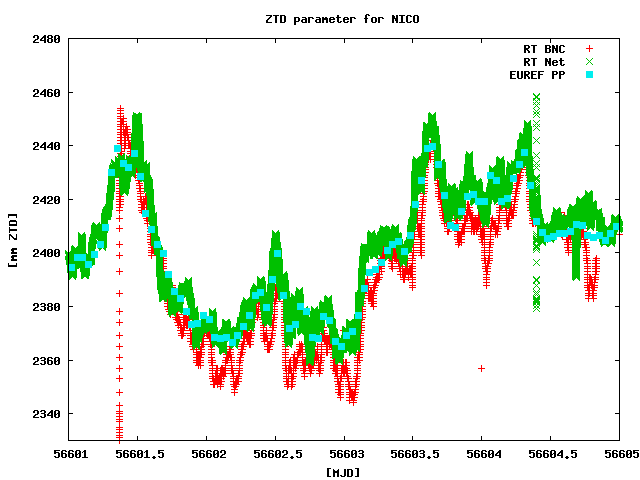
\includegraphics[width=0.9\textwidth,angle=0]{tropo3.png}
  \end{center}
\end{frame}

%%%%%%%%%%%%%%%%%%%%%%%%%%%%%%%%%%%%%%%%%%%%%%%%%%%%%%%%%%%%%%%%%%%%%%%%%%%%%%%%

\begin{frame}
  \frametitle{Principle of our PPP-RTK Algorithm}
  For a dual-band GPS receiver, the observation equations may read as
  \begin{eqnarray*}
  P^i & = & \varrho^i + c\;\delta - c\;\delta^i + T^i + b_P              \\
  L^i & = & \varrho^i + c\;\delta - c\;\delta^i + T^i + b^i
  \end{eqnarray*}
  where
  \begin{tabbing}
  $P^i$, $L^i$ ~~~~~~~ \= are the ionosphere-free code and phase measurements, \\ 
  $\varrho^i$          \> is the travel distance between the satellite 
                          and the receiver,                               \\
  $\delta$, $\delta^i$ \> are the receiver and satellite clock errors,    \\
  $T^i$                \> is the tropospheric delay,                      \\
  $b_P$                \> is the code bias, and                           \\
  $b^i$                \> is the phase bias (including initial
                          phase ambiguity).
  \end{tabbing}
  The single-difference bias $b^{ij} = b^i - b^j$ is given by
  \begin{displaymath}
  b^{ij} = \displaystyle\frac{\lambda_5-\lambda_3}{2}\;(n_5^{ij} + b_5^{ij})
              + \lambda_3\;(n_1^{ij} + b_1^{ij}) 
  \end{displaymath}
   where
  \begin{tabbing}
  $n_1^{ij}$, $n_5^{ij}$ ~~~~ \= are the narrow-lane and wide-lane integer ambiguities \\
  $b_1^{ij}$                 \> is the narrow-lane (receiver-independent) SD bias \\
  $b_5^{ij}$                 \> is the wide-lane (receiver-independent) SD bias
  \end{tabbing}
\end{frame}

%%%%%%%%%%%%%%%%%%%%%%%%%%%%%%%%%%%%%%%%%%%%%%%%%%%%%%%%%%%%%%%%%%%%%%%%%%%%%%%%

\begin{frame}
  \frametitle{Principle of our PPP-RTK Algorithm (cont.)}
  Receiver-independent single-difference biases $b_1^{ij}$ and $b_5^{ij}$ have 
  to be estimated on the server-side.
  \begin{itemize}
  \item Narrow-lane bias $b_1^{ij}$ may be combined with satellite clock
    corrections $\Longrightarrow$ \textbf{modified satellite clock corrections.}
  \item Wide-lane bias have to be transmitted from the server to the client
    (this bias is stable in time and can thus be transmitted in lower rate).
  \end{itemize}

  On the client-side the biases $b_1^{ij}$ and $b_5^{ij}$ are used as known
  quantities. It allows fixing the integer ambiguities $n_5^{ij}$ and
  $n_1^{ij}$. The technique is called Precise Point Positioning with Ambiguity
  Resolution (PPP~AR) or PPP~RTK, or zero-difference ambiguity
  fixing (the latter term not fully correct because the ambiguities are
  actually being fixed on single-difference level).
\end{frame}

%%%%%%%%%%%%%%%%%%%%%%%%%%%%%%%%%%%%%%%%%%%%%%%%%%%%%%%%%%%%%%%%%%%%%%%%%%%%%%%%

\begin{frame}
  \frametitle{Performance}
  \begin{center}
    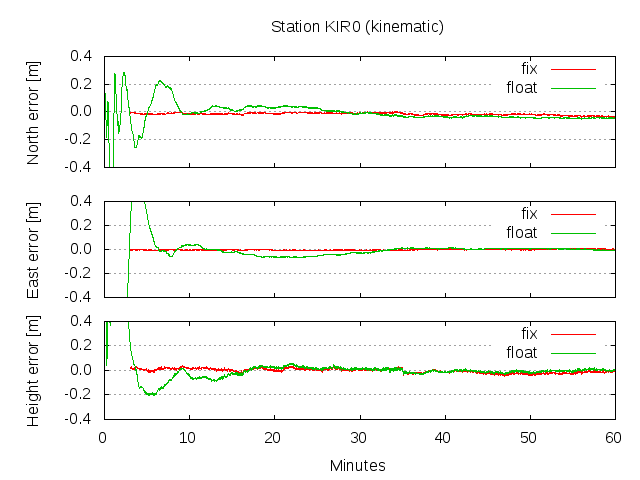
\includegraphics[width=0.75\textwidth]{kir0.png}
  \end{center}
  \vspace*{-5mm}
  \begin{block}{Standard deviations (N,E,U)}
  \vspace*{3mm}
  \begin{small}
  \hspace*{2cm}
  \begin{tabular}{l|ccc|ccc}
  \mbox{} & \multicolumn{3}{c|}{10-60 min} & \multicolumn{3}{c}{30-60 min} \\
  float & 0.034 & 0.026 & 0.026         & 0.010 & 0.009 & 0.011  \\
  fix   & 0.007 & 0.003 & 0.016         & 0.007 & 0.003 & 0.012
  \end{tabular}
  \end{small}
  \end{block}
\end{frame}

%%%%%%%%%%%%%%%%%%%%%%%%%%%%%%%%%%%%%%%%%%%%%%%%%%%%%%%%%%%%%%%%%%%%%%%%%%%%%%%%

\begin{frame}
  \frametitle{Challenges}
  PPP~RTK works and provides mm-accuracy results, what is this symposium
  about?

  \pause
  There are still both principal and technical problems and challenges:
  \begin{itemize}
  \item Principal problems:
    \begin{itemize}
    \item Convergence time: PPP~RTK in the form outlined above provides
      accuracy similar (or even slightly better) to RTK but the convergence
      time is longer.
    \item There is a degradation in accuracy with the age of corrections.
    \item Glonass ambiguity resolution: is it possible to resolve Glonass
      ambiguities? (yes, it is possible but it implicates introducing new
      parameters - does it really improve the results?)
    \item ...
    \end{itemize}
  \item Technical problems:
    \begin{itemize}
    \item Availability of data in real time (reference network, high-precision
          satellite orbits).
    \item Very high CPU requirements on the server-side.
    \item Solution robustness on the server-side 
          (problems with reliable DD ambiguity resolution). 
    \item ...
    \end{itemize}
  \end{itemize}
\end{frame}

%%%%%%%%%%%%%%%%%%%%%%%%%%%%%%%%%%%%%%%%%%%%%%%%%%%%%%%%%%%%%%%%%%%%%%%%%%%%%%%%

\begin{frame}
  \frametitle{Challenges (cont.)}
  \begin{block}{Longer convergence time}
  In case of a standard RTK the very short convergence time is being achieved
  thanks to the combined DD ambiguity resolution on both $L_1$ and $L_2$ when
  the differential ionospheric bias can either be neglected (short baselines)
  or its influence is mitigated (stochastic ionosphere estimation with
  constraints).

  On the contrary, the outlined PPP~RTK algorithm is in principle based on
  processing single (ionosphere-free) linear combination and resolving only
  one set of (narrow-lane) initial phase ambiguities.
  \end{block}
  \begin{block}{Possible solutions}
  \begin{itemize}
  \item third carrier
  \item multiple GNSS (Glonass ambiguity resolution?)
  \item processing original carriers (instead of ionosphere-free linear
    combination) and modeling the ionosphere?
  \item ?
  \end{itemize}
  \end{block}
\end{frame}

%%%%%%%%%%%%%%%%%%%%%%%%%%%%%%%%%%%%%%%%%%%%%%%%%%%%%%%%%%%%%%%%%%%%%%%%%%%%%%%%

\begin{frame}
  \frametitle{Challenges (cont.)}
  \begin{block}{Age of corrections 0 s}
  \begin{center}
    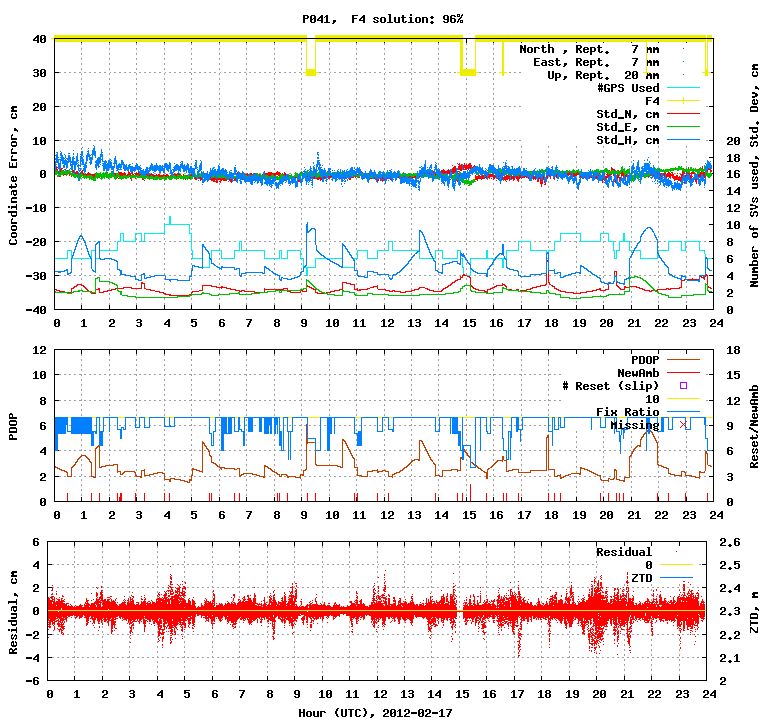
\includegraphics[width=0.6\textwidth]{age1.png}
  \end{center}
  \end{block}
\end{frame}

%%%%%%%%%%%%%%%%%%%%%%%%%%%%%%%%%%%%%%%%%%%%%%%%%%%%%%%%%%%%%%%%%%%%%%%%%%%%%%%%

\begin{frame}
  \frametitle{Challenges (cont.)}
  \begin{block}{Age of corrections up to 35 s}
  \begin{center}
    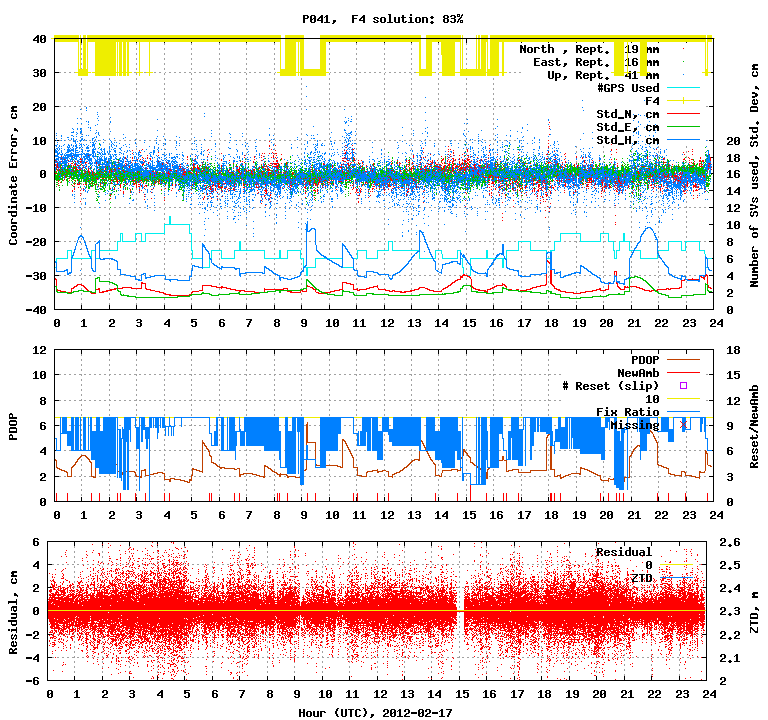
\includegraphics[width=0.6\textwidth]{age2.png}
  \end{center}
  \end{block}
\end{frame}

%%%%%%%%%%%%%%%%%%%%%%%%%%%%%%%%%%%%%%%%%%%%%%%%%%%%%%%%%%%%%%%%%%%%%%%%%%%%%%%%

\begin{frame}
  \frametitle{Real-Time Data Availability}
  \framesubtitle{IGS network: very good global coverage:}
  \vspace*{-5.5cm}
  \begin{center}
    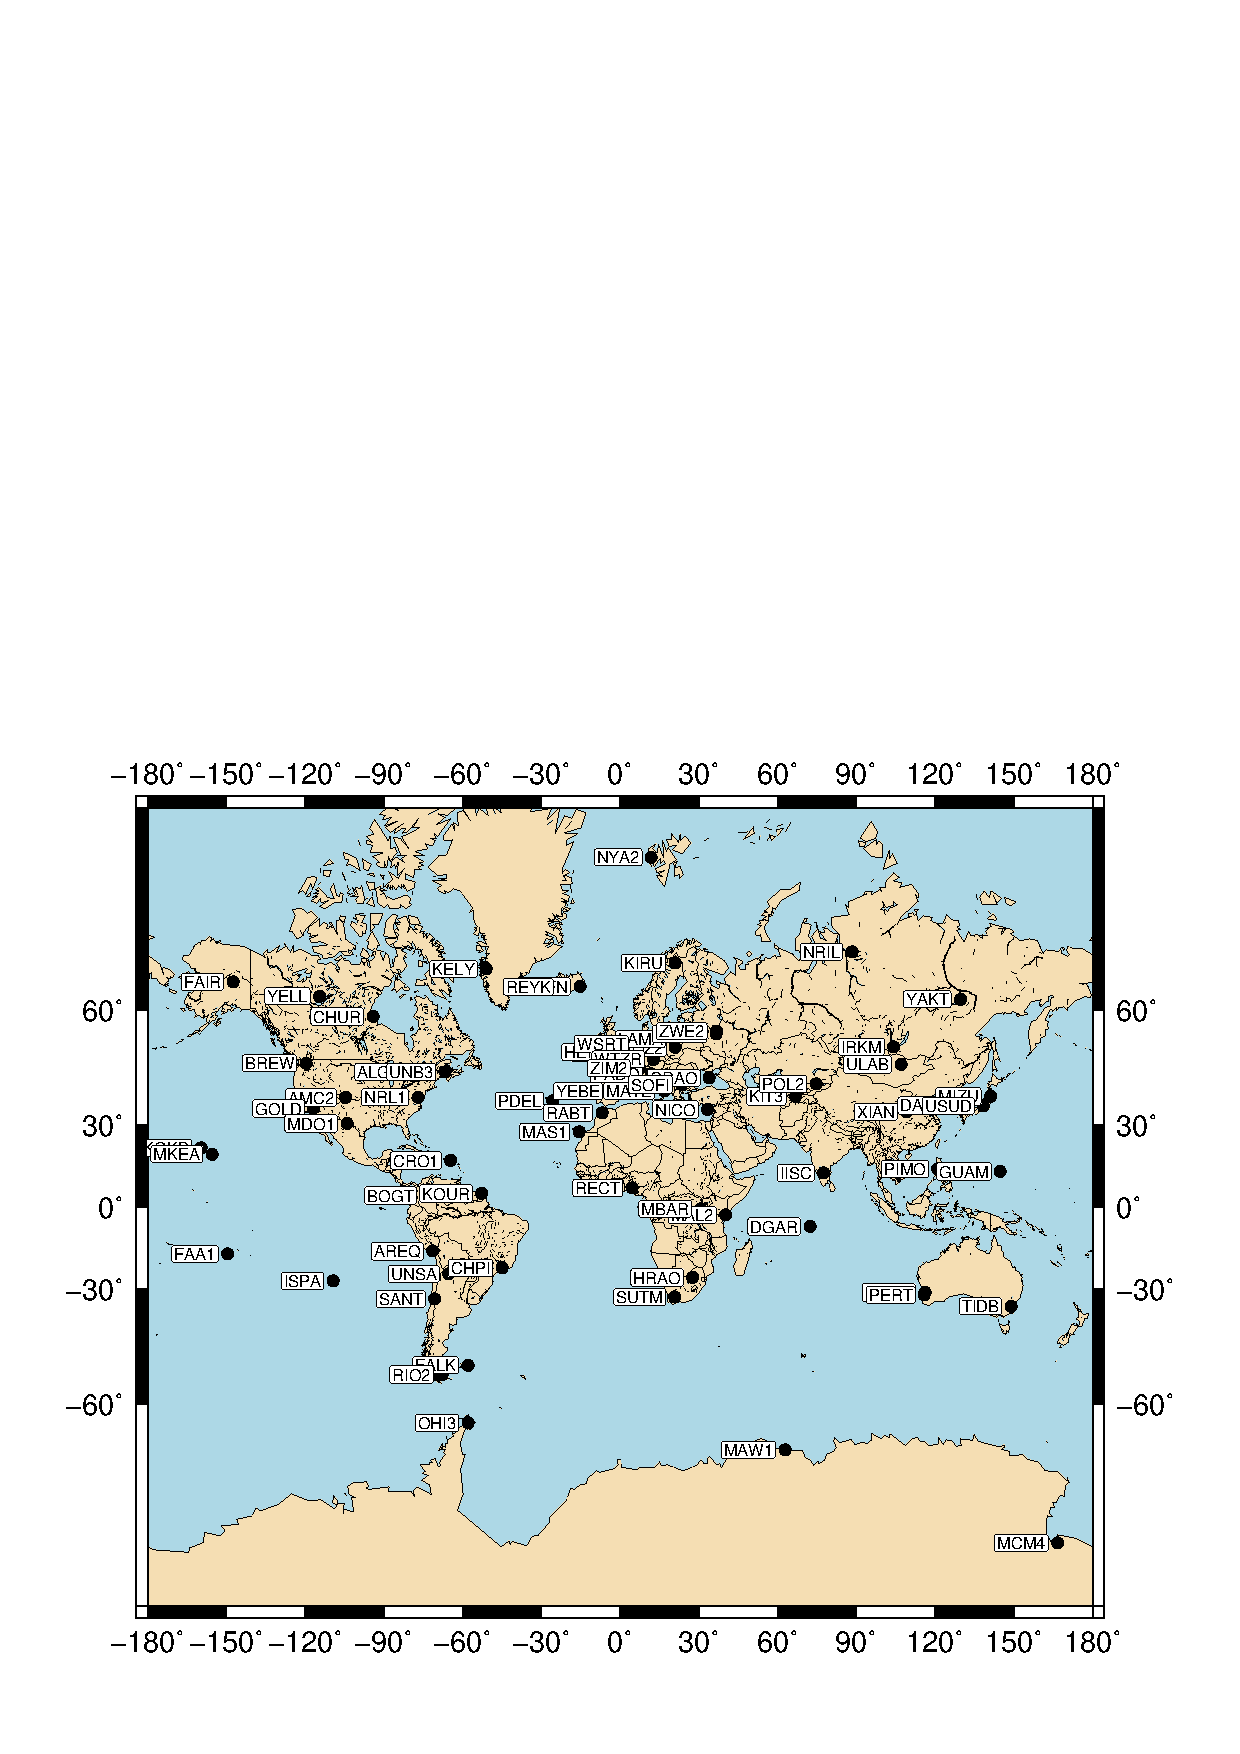
\includegraphics[width=0.9\textwidth]{map.pdf}
  \end{center}
\end{frame}

%%%%%%%%%%%%%%%%%%%%%%%%%%%%%%%%%%%%%%%%%%%%%%%%%%%%%%%%%%%%%%%%%%%%%%%%%%%%%%%%

\begin{frame}
  \frametitle{Real-Time Data Availability (cont.)}
  \begin{tabular}{cc}
  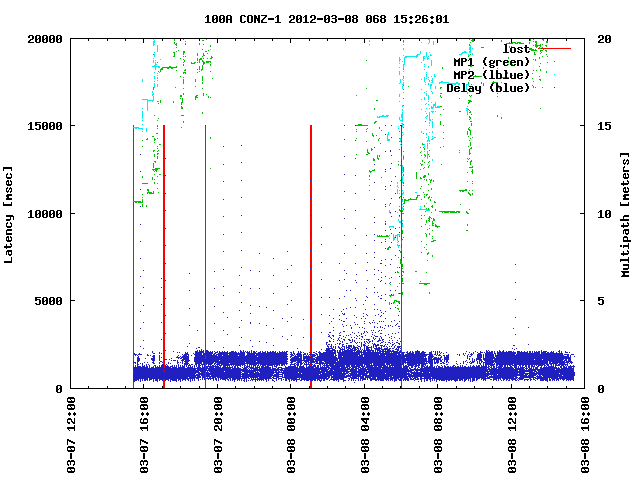
\includegraphics[width=0.4\textwidth]{100A_lat.png} &
  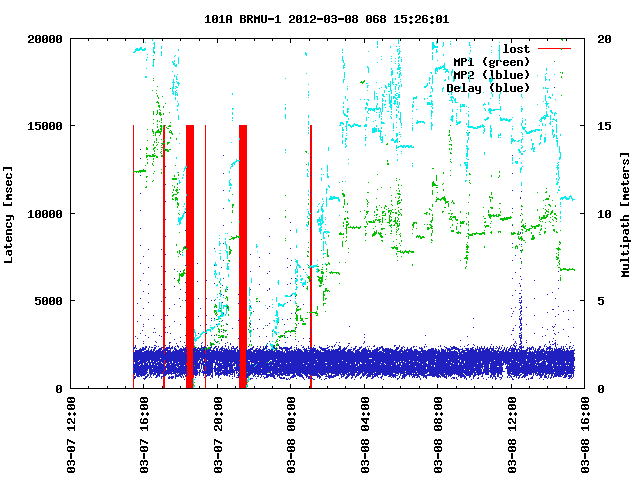
\includegraphics[width=0.4\textwidth]{101A_lat.png} \\
  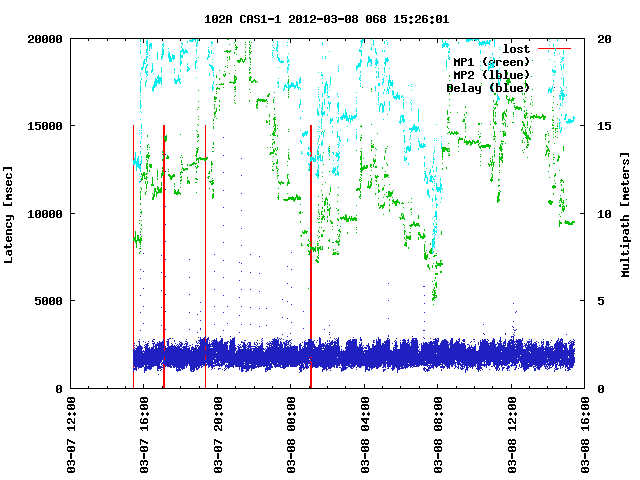
\includegraphics[width=0.4\textwidth]{102A_lat.png} &
  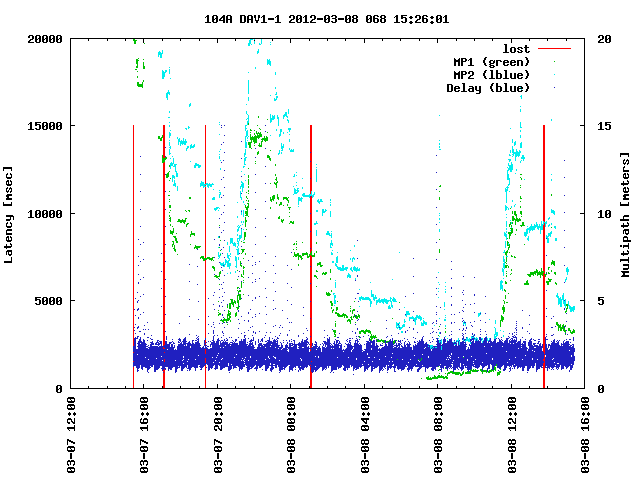
\includegraphics[width=0.4\textwidth]{104A_lat.png}
  \end{tabular}

  Gaps in reference network data may degrade the PPP~RTK server performance
  considerably!
\end{frame}

%%%%%%%%%%%%%%%%%%%%%%%%%%%%%%%%%%%%%%%%%%%%%%%%%%%%%%%%%%%%%%%%%%%%%%%%%%%%%%%%

\begin{frame}
  \frametitle{Technical issues}
  \begin{block}{CPU-requirements on the server-side}
  Processing a global reference network is a very CPU-intensive
  task. Numerically stable forms of the Kalman filter (square-root, UDU
  factorization etc.) require very fast hardware. 

  Possible solutions:
  \begin{itemize}
  \item Processing optimization (estimating various kinds of parameters in 
        different rates)
  \item Parallel processing 
  \item Advanced hardware (GPS Solutions uses GPU-accelerated library)
  \end{itemize}
  \end{block}
  \begin{block}{Reliable DD ambiguity resolution on the server-side}
  Reliable double-difference ambiguity resolution on the server-side remains
  the crucial issue of the PPP~RTK technique.
  \end{block}
  \begin{block}{Dissemination of PPP~RTK corrections}
  \begin{itemize}
  \item data links
  \item formats (standardization?)
  \item optimization of correction rates (bandwidth)
  \end{itemize}
  \end{block}
\end{frame}

%%%%%%%%%%%%%%%%%%%%%%%%%%%%%%%%%%%%%%%%%%%%%%%%%%%%%%%%%%%%%%%%%%%%%%%%%%%%%%%%

\begin{frame}
  \frametitle{Satellite orbits}

  Predicted part of the IGS ultra-rapid orbits (available in real-time) is
  sometimes not sufficient for the processing of a global reference network
  (with narrow-lane ambiguity resolution). We have been forced to implement
  the real-time orbit determination capability in our main processing tool
  RTNet (Real-Time Network software).
  \begin{center}
    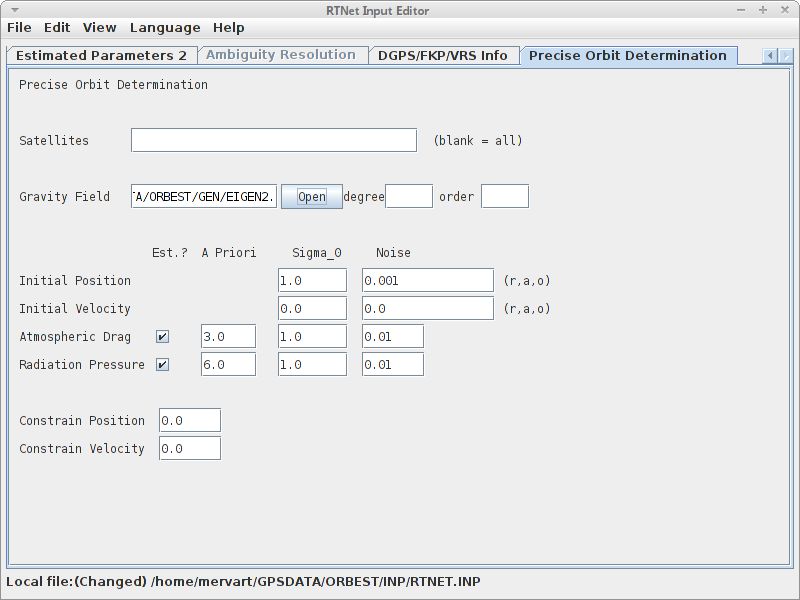
\includegraphics[width=0.75\textwidth]{rtnet_pod.png}
  \end{center}
\end{frame}

%%%%%%%%%%%%%%%%%%%%%%%%%%%%%%%%%%%%%%%%%%%%%%%%%%%%%%%%%%%%%%%%%%%%%%%%%%%%%%%%

\begin{frame}
  \frametitle{Regional versus global PPP~RTK services} 
  Currently we are routinely running both regional and global PPP~RTK service
  demonstrators in real-time (some of the results will be shown below).
  \begin{itemize}
  \item in principal there is no difference between a global and regional
    service as far as the data processing, algorithms etc. is concerned
  \item global PPP~RTK service has at least the following two advantages
     \begin{itemize}
     \item[1.] a single correction stream can serve all users
     \item[2.] all satellites are tracked permanently (helps ambiguity 
               resolution)
     \end{itemize}
  \item global PPP~RTK service is much more challenging (data availability,
    CPU-requirements on the server-side, DD ambiguity resolution on long
    baselines, the highest requirements for the accuracy of the satellite
    orbits)
  \end{itemize}

\end{frame}

%%%%%%%%%%%%%%%%%%%%%%%%%%%%%%%%%%%%%%%%%%%%%%%%%%%%%%%%%%%%%%%%%%%%%%%%%%%%%%%%

\begin{frame}
  \frametitle{Services monitoring} 
  Reliable, production-quality PPP~RTK service requires sophisticated
  monitoring tools.
  \begin{tabular}{cc}
  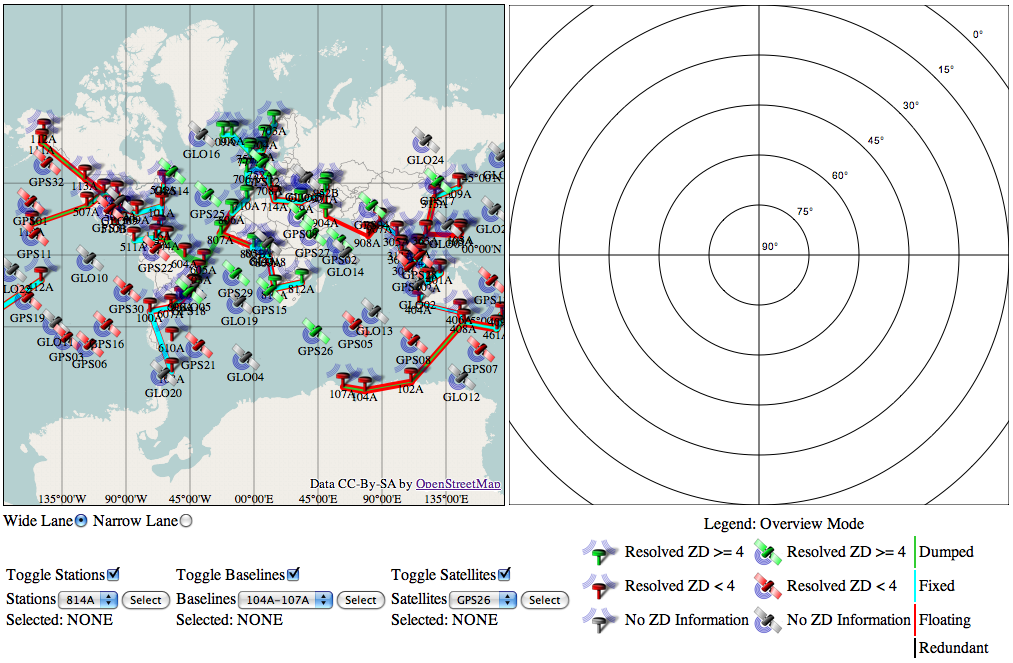
\includegraphics[width=0.6\textwidth]{monitor1.png} & \\[-1.5cm]
  & \hspace*{-3cm} 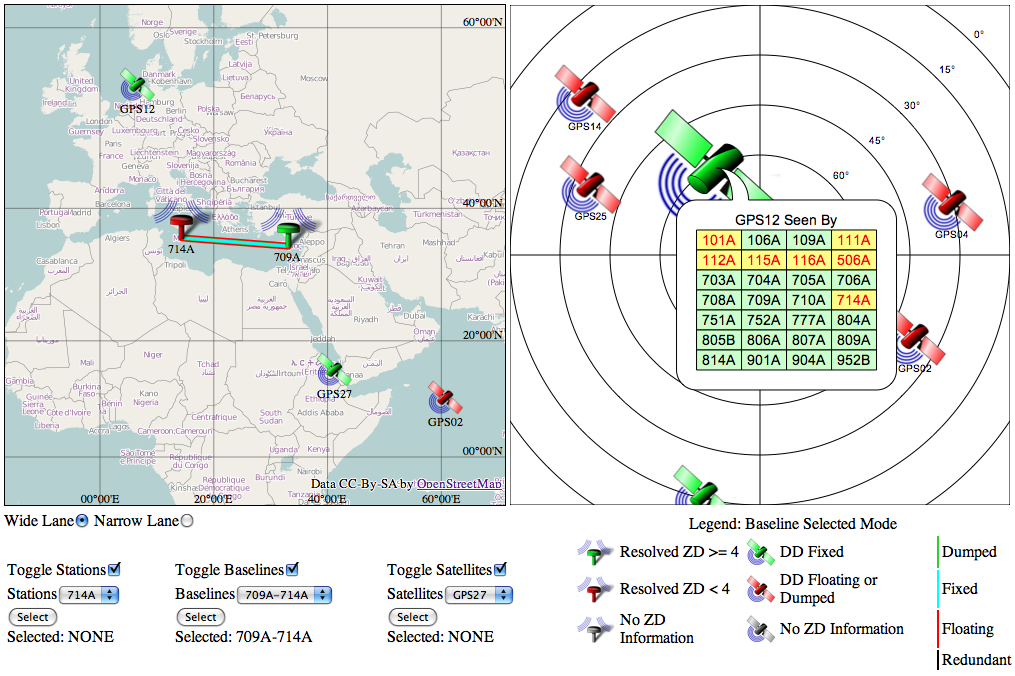
\includegraphics[width=0.6\textwidth]{monitor2.png}
  \end{tabular}

\end{frame}

%%%%%%%%%%%%%%%%%%%%%%%%%%%%%%%%%%%%%%%%%%%%%%%%%%%%%%%%%%%%%%%%%%%%%%%%%%%%%%%%

\begin{frame}
  \frametitle{Results}
  \begin{center}
    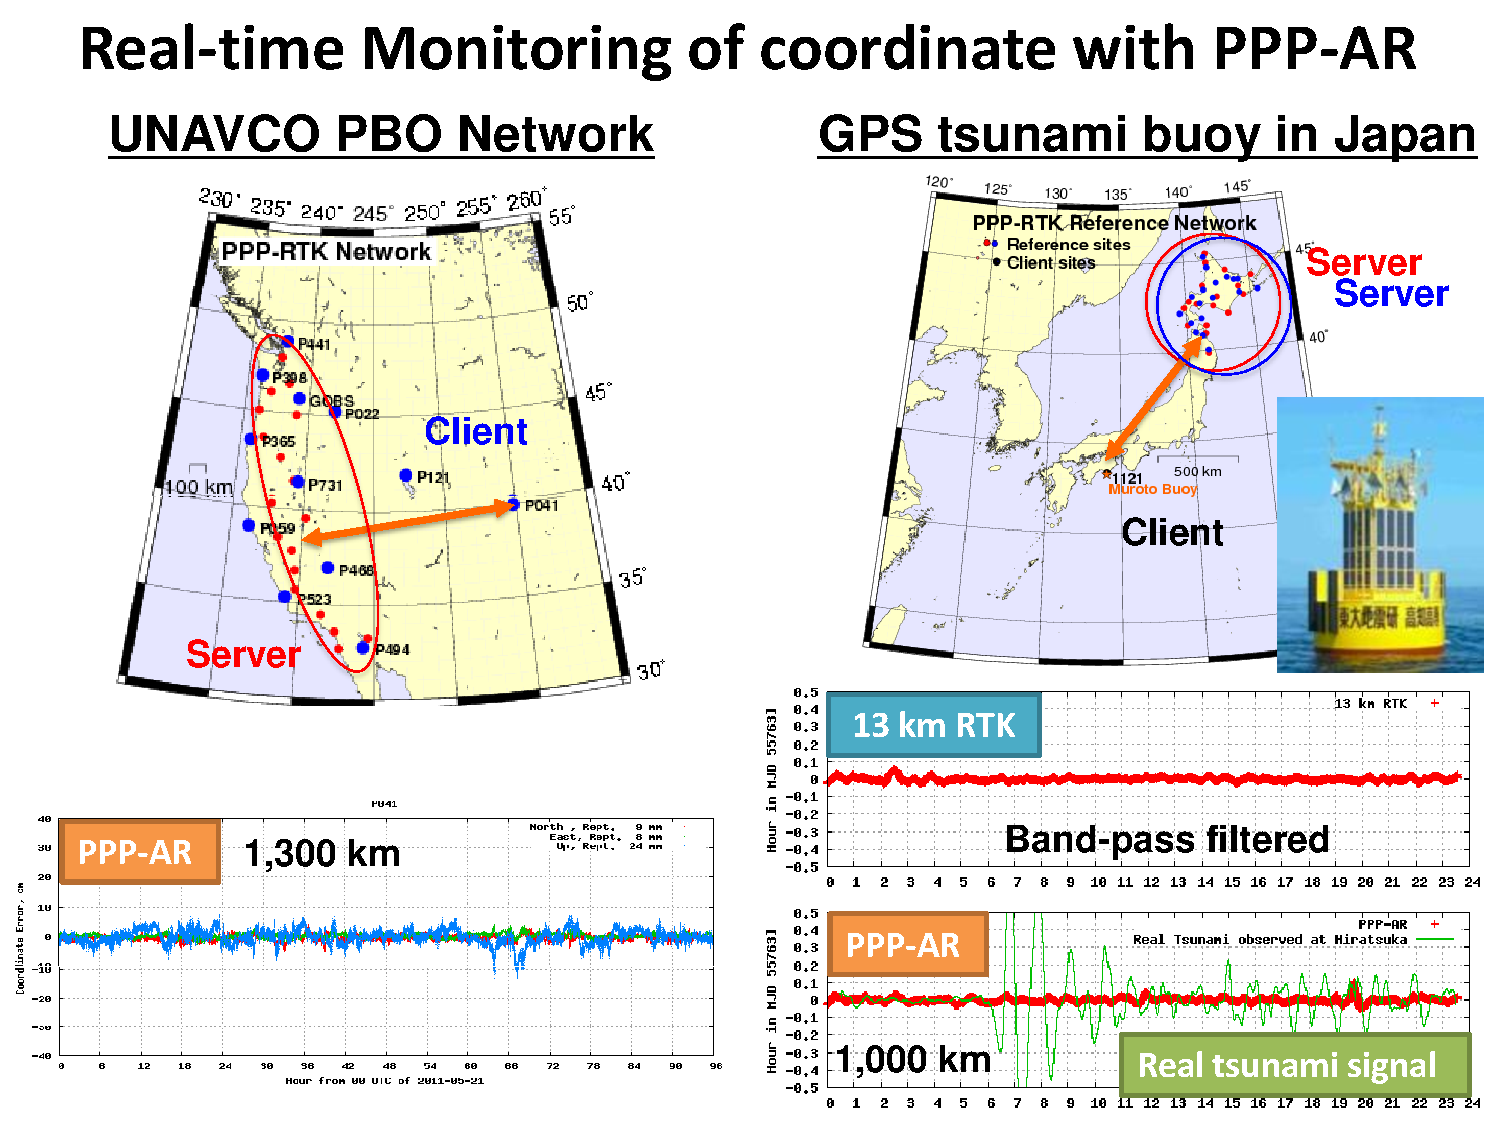
\includegraphics[width=0.9\textwidth]{tsunami.pdf}
  \end{center}
\end{frame}

%%%%%%%%%%%%%%%%%%%%%%%%%%%%%%%%%%%%%%%%%%%%%%%%%%%%%%%%%%%%%%%%%%%%%%%%%%%%%%%%

\begin{frame}
  \frametitle{Results (cont.)}
  \begin{center}
    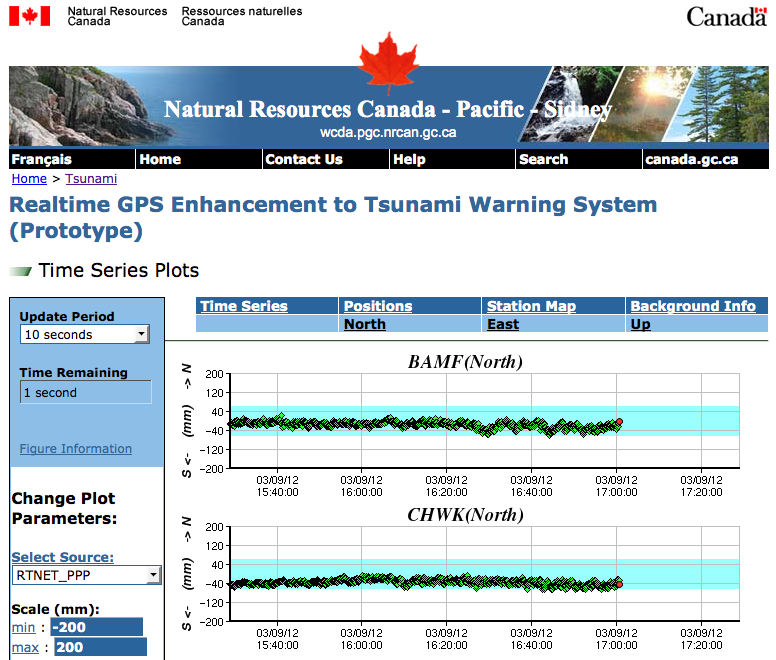
\includegraphics[width=0.9\textwidth]{nrcan.png}
  \end{center}
\end{frame}

\end{document}
